\documentclass[12pt, letterpaper]{article}
\usepackage[margin=1in]{geometry}
\usepackage{mathptmx}
\usepackage{amsmath}
\usepackage{graphicx}
\usepackage{booktabs}
\usepackage{multirow}
\usepackage[font={small,it}, justification=centering, labelfont=bf]{caption}
\usepackage{float}
\usepackage[skip=4pt]{parskip}
\usepackage{hyperref}
\hypersetup{colorlinks=true, linkcolor=blue, urlcolor=blue}
\usepackage{tikz}
\usetikzlibrary{automata, positioning, arrows.meta}
\usepackage{titlesec}
\titlespacing*{\section}{0pt}{8pt}{4pt}
\titlespacing*{\subsection}{0pt}{6pt}{2pt}
% Roman numeral section counter
\renewcommand{\thesection}{\Roman{section}}
\titleformat{\section}{\normalfont\bfseries\large}{\thesection.}{0.5em}{}

% Simple arabic numbering for subsections
\renewcommand{\thesubsection}{\arabic{subsection}}
\titleformat{\subsection}{\normalfont\bfseries}{\thesubsection.}{0.5em}{}

\begin{document}

\begin{center}
  {\Large \textbf{Report for CDA 3201L Lab \#8}}\\[10pt]
  {\large \textbf{Sequential Circuits -- FSM Design (Vending Machine Controller)}}\\[20pt]
  \begin{tabular}{ll}
    \textbf{Name:} Tuan Khang Phan & \textbf{UID:} U30382645 \\[4pt]
    \textbf{Name:} Huu Phat Nguyen & \textbf{UID:} U46082380 \\
  \end{tabular}
\end{center}

% ─────────────────────────────────────────────
\section{Introduction}

The purpose of this lab is to practice turning an informal specification into a finite-state
machine (FSM) design and a working sequential circuit.  We designed and implemented a
simple vending machine controller that accepts nickels (5\,cents) and dimes (10\,cents)
through a single coin slot.  Two sensor inputs, $N$ (nickel) and $D$ (dime), indicate which
coin was detected.  When the accumulated credit reaches 25\,cents, the controller asserts a
\textit{vend} output and dispenses candy; the specification states that the machine does not
return change, so any coin that brings the total to 25\,cents or beyond triggers a vend and
returns the FSM to the idle (0\,cents) state.  The implementation uses flip-flops for state,
combinational logic for next-state and outputs, a 7-segment display to show the current state
(or an agreed encoding of the credit), an LED for the vend condition, and an asynchronous
active-low reset.

% ─────────────────────────────────────────────
\section{Methods and Materials}

We used the following components and equipment (exact IC mix depends on the chosen flip-flop
type after comparing D vs.\ JK realizations):

\begin{itemize}
  \item Flip-flop IC(s) for state registers (e.g.\ SN74LS74 dual D-type, or SN74LS109 dual JK
        configured as D if needed)
  \item Combinational logic ICs as required by the minimized equations (e.g.\ SN74LS00 quad
        NAND, SN74LS04 hex inverter, additional NAND/AND packages for NAND--NAND form)
  \item SN74LS47N BCD-to-7-segment decoder/driver and common-anode 7-segment display (current
        limiting resistors on segment lines)
  \item One LED and resistor for the \textit{vend} output
  \item Tactile switches or debounced inputs to emulate $N$ and $D$ (with pull-up or pull-down
        resistors as appropriate for active-high or active-low sensing)
  \item Push button and pull-up for asynchronous $\overline{\text{CLR}}$ reset
  \item Breadboard, jumper wires, 5\,V supply
  \item Function generator (0.5\,Hz square wave, CMOS output) used as a slow ``step'' clock for
        demonstration, as in previous labs
\end{itemize}

We derived the state diagram and state table from the word specification, checked for
redundant states, chose a state assignment, minimized next-state and output logic (exploiting
don't-cares where valid), compared D vs.\ JK flip-flop realizations to minimize package count,
converted two-level SOP to NAND--NAND where required, drew a block diagram with IC pin-level
intent, and obtained TA approval before wiring.  After breadboarding, we verified transitions
under the slow clock and demonstrated operation to the TA.

% ─────────────────────────────────────────────
\section{Results}

\subsection{State Diagram (Lab Question 1)}

We model credit in 5\,cent steps.  Let the states represent totals of
$0,\,5,\,10,\,15,\,20$ cents before vending.  A nickel asserts $N$ and adds 5\,cents; a dime
asserts $D$ and adds 10\,cents.  We assume $N$ and $D$ are not asserted simultaneously (the
sensor resolves one coin at a time); the $ND{=}11$ input combination is treated as a
don't-care for next-state minimization.  When a coin would meet or exceed 25\,cents, the FSM
outputs \textit{vend} and returns to $0$\,cents (no change returned).

\begin{figure}[H]
\centering
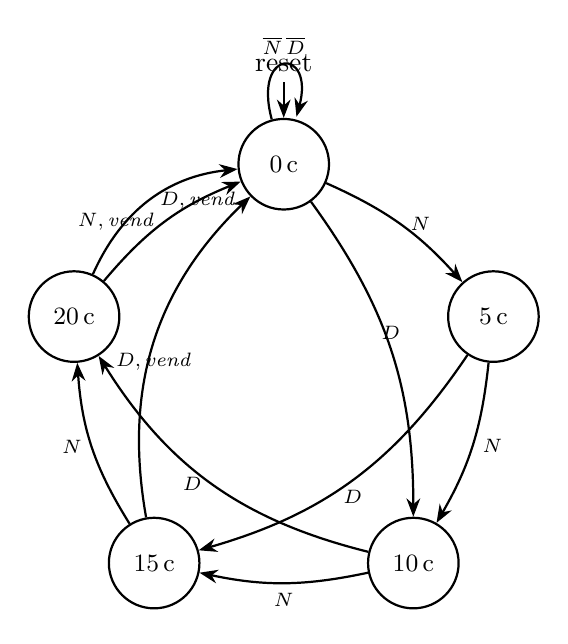
\begin{tikzpicture}[->, >=Stealth, thick,
    every state/.style={minimum size=1.15cm, font=\small}]

  \node[state, initial, initial text=reset, initial where=above]
    (s0) at (90:2.8cm)  {$0$\,c};
  \node[state]
    (s1) at (18:2.8cm)  {$5$\,c};
  \node[state]
    (s2) at (-54:2.8cm) {$10$\,c};
  \node[state]
    (s3) at (-126:2.8cm){$15$\,c};
  \node[state]
    (s4) at (162:2.8cm) {$20$\,c};

  % Self-loops on no coin (implicit in Moore formulation) omitted for clarity;
  % transitions labeled with (N), (D), or both outcomes

  \path (s0) edge [loop above] node[above, font=\scriptsize] {$\overline{N}\,\overline{D}$} (s0)
        (s0) edge [bend left=12] node[right, font=\scriptsize] {$N$} (s1)
        (s0) edge [bend left=18] node[above, font=\scriptsize] {$D$} (s2);

  \path (s1) edge [bend left=12] node[right, font=\scriptsize] {$N$} (s2)
        (s1) edge [bend left=20] node[below, font=\scriptsize] {$D$} (s3);

  \path (s2) edge [bend left=12] node[below, font=\scriptsize] {$N$} (s3)
        (s2) edge [bend left=22] node[left, font=\scriptsize] {$D$} (s4);

  \path (s3) edge [bend left=14] node[left, font=\scriptsize] {$N$} (s4)
        (s3) edge [bend left=28] node[below, font=\scriptsize] {$D$,\,\textit{vend}} (s0);

  \path (s4) edge [bend left=14] node[left, font=\scriptsize] {$N$,\,\textit{vend}} (s0)
        (s4) edge [bend left=30] node[right, font=\scriptsize] {$D$,\,\textit{vend}} (s0);

\end{tikzpicture}
\caption{State diagram for the vending controller.  States are labeled with accumulated credit.
A dime from 15\,cents or either a nickel from 20\,cents or a dime from 20\,cents reaches
$\geq 25$\,cents, asserts \textit{vend}, and returns to 0\,cents.}
\end{figure}

\subsection{State Table and State Minimization (Lab Question 2)}

Let Moore outputs be: 7-segment encoding of the current state (see subsection below) and a
\textit{vend} LED that your TA-approved schematic defines (Moore output in some states, or a
one-cycle Mealy pulse on the qualifying coin---stay consistent with your state diagram).

\begin{center}
\small
\begin{tabular}{|c|cc|c|c|}
  \hline
  \textbf{Present} & \multicolumn{2}{c|}{\textbf{Inputs}} &
  \textbf{Next total} & \textbf{Notes} \\
  total (c) & $N$ & $D$ & (c) & \\
  \hline
  0 & 0 & 0 & 0 & hold \\
  0 & 1 & 0 & 5 & \\
  0 & 0 & 1 & 10 & \\
  0 & 1 & 1 & $d$ & don't-care ($N,D$ together) \\
  \hline
  5 & 0 & 0 & 5 & hold \\
  5 & 1 & 0 & 10 & \\
  5 & 0 & 1 & 15 & \\
  5 & 1 & 1 & $d$ & don't-care \\
  \hline
  10 & 0 & 0 & 10 & hold \\
  10 & 1 & 0 & 15 & \\
  10 & 0 & 1 & 20 & \\
  10 & 1 & 1 & $d$ & don't-care \\
  \hline
  15 & 0 & 0 & 15 & hold \\
  15 & 1 & 0 & 20 & \\
  15 & 0 & 1 & 0 & vend (25\,c); no change \\
  15 & 1 & 1 & $d$ & don't-care \\
  \hline
  20 & 0 & 0 & 20 & hold \\
  20 & 1 & 0 & 0 & vend (25\,c) \\
  20 & 0 & 1 & 0 & vend (30\,c total; no change) \\
  20 & 1 & 1 & $d$ & don't-care \\
  \hline
\end{tabular}
\end{center}

Here $d$ denotes don't-care for the illegal simultaneous $N{=}D{=}1$ assumption.  The five
totals $0,5,10,15,20$ are pairwise distinguishable by input sequences, so there are no
equivalent states to merge; five states is minimal for this abstraction.

\subsection{State Assignment, Excitation Equations, and D vs.\ JK (Lab Question 3)}

We require at least three state variables $y_2y_1y_0$ to encode five states.  One convenient
assignment maps the credit in nickels ($0\ldots 4$) to binary:

\begin{center}
\begin{tabular}{@{}ccc@{}}
  \toprule
  $(y_2,y_1,y_0)$ & Total credit & 7-seg digit \\
  \midrule
  000 & 0\,c (idle) & 0 \\
  001 & 5\,c & 1 \\
  010 & 10\,c & 2 \\
  011 & 15\,c & 3 \\
  100 & 20\,c & 4 \\
  \bottomrule
\end{tabular}
\end{center}

Unused code $101,110,111$ are don't-cares for logic minimization if the FSM is guaranteed to
reset into 000.  The 7-segment display can be driven by treating $(y_2,y_1,y_0)$ as a BCD value
$0\ldots 4$ with $D_{\text{MSB}}$ tied low on the SN74LS47N (same hookup style as prior labs),
so the display shows the state's ``nickel count'' $0$--$4$.

\medskip
\noindent\textbf{D flip-flops.} With DFFs, $Y_i = y_i^+$ (next state) for each bit.  Fill in a
Karnaugh map for each $Y_i$ from the encoded state table (rows: present $y_2y_1y_0$; columns:
$ND \in \{00,01,11,10\}$ or Gray-ordered $00,01,11,10$).  Use $d$ entries for unused present
states and for $ND{=}11$.  Sum-of-products expressions are then implemented in NAND--NAND
form using SN74LS00 (and inverters as needed).

\medskip
\noindent\textbf{JK flip-flops.} For each bit, use the JK excitation table to translate
$(y_i \rightarrow y_i^+)$ into $(J_i,K_i)$, then K-map $J_i$ and $K_i$ separately.  JK can
sometimes save gates when $J_i \neq K_i$ allows merging; compare total gate and IC count
against the D solution and document which option uses fewer ICs for your specific equations.

\medskip
\noindent\textbf{Vend output.} Combinational \textit{Vend} can be written as a sum of
minterms corresponding to the dime-from-15, nickel-from-20, and dime-from-20 transitions,
then minimized and NAND--NANDed.  Tie the vend LED through a current-limiting resistor.

\medskip
\noindent\textbf{Required I/O checklist.}
\begin{itemize}
  \item Two inputs $N$ and $D$ with appropriate pull-ups/downs and debouncing if switches are
        used to emulate the coin sensors.
  \item Active-low asynchronous $\overline{\text{CLR}}$ on all flip-flops tied to a reset
        button (pull-up to $V_{DD}$), with $\overline{\text{PRE}}$ disabled per datasheet.
  \item SN74LS47N (or agreed variant) plus common-anode display showing the encoded state
        $0\ldots 4$.
  \item One LED showing the \textit{vend} condition.
\end{itemize}

\subsection{Block Diagram, NAND--NAND, and TA Sign-Off (Lab Question 4)}

Figure~\ref{fig:block} is a representative block diagram: registers (three FFs), next-state
logic block, output logic for \textit{Vend}, and display decoder.  Replace generic labels
with your final chip list and pin-level nets after minimization.  For every two-level SOP
network, duplicate De Morgan with NANDs for NAND--NAND realization.  Attach a copy of the
TA-approved schematic in your submission package if required by your section.

\begin{figure}[H]
\centering
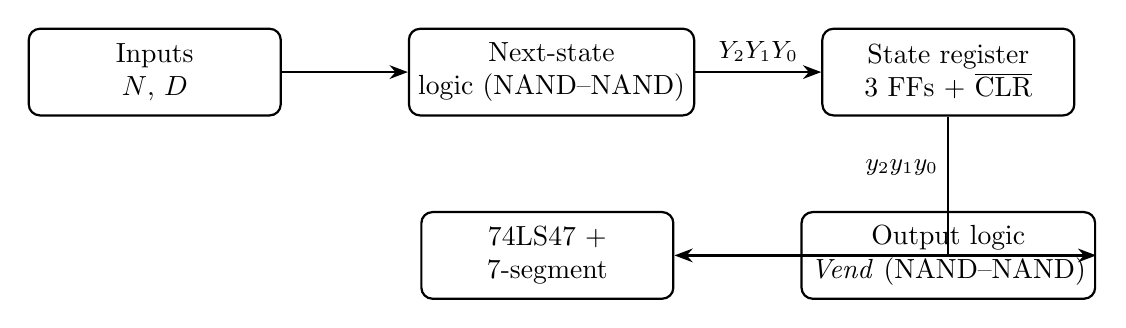
\begin{tikzpicture}[>=Stealth, thick, block/.style={draw, rounded corners, minimum width=3.2cm,
    minimum height=1.1cm, align=center}, line/.style={->}]

  \node[block] (in) {Inputs\\$N$, $D$};
  \node[block, right=1.6cm of in] (ns) {Next-state\\logic (NAND--NAND)};
  \node[block, right=1.6cm of ns] (reg) {State register\\3 FFs + $\overline{\text{CLR}}$};
  \node[block, below=1.2cm of reg] (out) {Output logic\\\textit{Vend} (NAND--NAND)};
  \node[block, left=1.6cm of out] (seg) {74LS47 +\\7-segment};

  \draw[line] (in) -- node[above, font=\small] {} (ns);
  \draw[line] (ns) -- node[above, font=\small] {$Y_2Y_1Y_0$} (reg);
  \draw[line] (reg.south) |- node[above left, font=\small, pos=0.25] {$y_2y_1y_0$} (out.east);
  \draw[line] (reg.south) |- (seg.east);

\end{tikzpicture}
\caption{High-level block diagram for the vending FSM.  Clock (0.5\,Hz demo) connects to all
flip-flops; reset and power distribution are omitted for clarity.}
\label{fig:block}
\end{figure}

\subsection{Experimental Procedure and Observations}

Following the lab handout, we configured the function generator for a 0.5\,Hz CMOS square
wave as the clock, wired the approved design on the breadboard, and stepped through
representative coin sequences (e.g.\ nickel sequences to 25\,cents, dime shortcuts, and
over-threshold cases that still vend with no change returned).  We verified that the display
tracks the credited total in the agreed encoding and that the vend LED asserts only on valid
25\,cents events.

\begin{figure}[H]
\centering
\fbox{\parbox[c][4.2cm][c]{0.72\linewidth}{\centering
\small (Replace with photo of your breadboard: FFs, NAND logic, 7-segment, vend LED, clock,
reset, and $N$/$D$ switches.)}}
\caption{Breadboard implementation of the vending machine controller (placeholder).}
\end{figure}

% Optional: uncomment when you export screenshots from your HDL/simulation tool
% \begin{figure}[H]
% \centering
% \includegraphics[width=0.72\linewidth]{vending_fsm_tb.png}
% \caption{Optional simulation waveform for key test vectors.}
% \end{figure}

% ─────────────────────────────────────────────
\section{Discussion}

The five-state credit model matches the specification that only multiples of five and ten
cents are inserted and that vending occurs exactly at 25\,cents with no change.  Treating
$ND{=}11$ as a don't-care reflects a single-slot sensor assumption and simplifies logic.
Displaying state as $0$--$4$ ``nickel units'' keeps the 7-segment interface simple with a
single SN74LS47N digit.

Comparing D and JK realizations is problem-dependent: DFFs give $D_i = Y_i$ directly, while JK
maps may merge $J$ and $K$ terms across bits.  The winner is whichever meets timing with the
fewest packages in your mapped equations---document the gate counts you actually built.

Breadboard errors (floating inputs, swapped $Q/\overline{Q}$, incorrect CLR polarity) were the
main debug issues; the slow 0.5\,Hz clock made state transitions easy to follow visually.

% ─────────────────────────────────────────────
\section{Conclusion}

We derived a minimal vending-machine FSM accepting nickels and dimes, tabulated next states,
encoded five credit states in three bits, minimized logic with don't-cares, planned
NAND--NAND implementation and display interfacing, and verified the circuit experimentally under
a 0.5\,Hz clock.  The design meets the lab I/O requirements: $N$ and $D$, asynchronous reset,
7-segment state display, and a vend LED.

\end{document}
